% Options for packages loaded elsewhere
\PassOptionsToPackage{unicode}{hyperref}
\PassOptionsToPackage{hyphens}{url}
%
\documentclass[
]{book}
\usepackage{amsmath,amssymb}
\usepackage{lmodern}
\usepackage{ifxetex,ifluatex}
\ifnum 0\ifxetex 1\fi\ifluatex 1\fi=0 % if pdftex
  \usepackage[T1]{fontenc}
  \usepackage[utf8]{inputenc}
  \usepackage{textcomp} % provide euro and other symbols
\else % if luatex or xetex
  \usepackage{unicode-math}
  \defaultfontfeatures{Scale=MatchLowercase}
  \defaultfontfeatures[\rmfamily]{Ligatures=TeX,Scale=1}
\fi
% Use upquote if available, for straight quotes in verbatim environments
\IfFileExists{upquote.sty}{\usepackage{upquote}}{}
\IfFileExists{microtype.sty}{% use microtype if available
  \usepackage[]{microtype}
  \UseMicrotypeSet[protrusion]{basicmath} % disable protrusion for tt fonts
}{}
\makeatletter
\@ifundefined{KOMAClassName}{% if non-KOMA class
  \IfFileExists{parskip.sty}{%
    \usepackage{parskip}
  }{% else
    \setlength{\parindent}{0pt}
    \setlength{\parskip}{6pt plus 2pt minus 1pt}}
}{% if KOMA class
  \KOMAoptions{parskip=half}}
\makeatother
\usepackage{xcolor}
\IfFileExists{xurl.sty}{\usepackage{xurl}}{} % add URL line breaks if available
\IfFileExists{bookmark.sty}{\usepackage{bookmark}}{\usepackage{hyperref}}
\hypersetup{
  pdftitle={Exploratory Data Analysis in the 21st Century},
  pdfauthor={Di Cook and Emi Tanaka},
  hidelinks,
  pdfcreator={LaTeX via pandoc}}
\urlstyle{same} % disable monospaced font for URLs
\usepackage{color}
\usepackage{fancyvrb}
\newcommand{\VerbBar}{|}
\newcommand{\VERB}{\Verb[commandchars=\\\{\}]}
\DefineVerbatimEnvironment{Highlighting}{Verbatim}{commandchars=\\\{\}}
% Add ',fontsize=\small' for more characters per line
\usepackage{framed}
\definecolor{shadecolor}{RGB}{248,248,248}
\newenvironment{Shaded}{\begin{snugshade}}{\end{snugshade}}
\newcommand{\AlertTok}[1]{\textcolor[rgb]{0.94,0.16,0.16}{#1}}
\newcommand{\AnnotationTok}[1]{\textcolor[rgb]{0.56,0.35,0.01}{\textbf{\textit{#1}}}}
\newcommand{\AttributeTok}[1]{\textcolor[rgb]{0.77,0.63,0.00}{#1}}
\newcommand{\BaseNTok}[1]{\textcolor[rgb]{0.00,0.00,0.81}{#1}}
\newcommand{\BuiltInTok}[1]{#1}
\newcommand{\CharTok}[1]{\textcolor[rgb]{0.31,0.60,0.02}{#1}}
\newcommand{\CommentTok}[1]{\textcolor[rgb]{0.56,0.35,0.01}{\textit{#1}}}
\newcommand{\CommentVarTok}[1]{\textcolor[rgb]{0.56,0.35,0.01}{\textbf{\textit{#1}}}}
\newcommand{\ConstantTok}[1]{\textcolor[rgb]{0.00,0.00,0.00}{#1}}
\newcommand{\ControlFlowTok}[1]{\textcolor[rgb]{0.13,0.29,0.53}{\textbf{#1}}}
\newcommand{\DataTypeTok}[1]{\textcolor[rgb]{0.13,0.29,0.53}{#1}}
\newcommand{\DecValTok}[1]{\textcolor[rgb]{0.00,0.00,0.81}{#1}}
\newcommand{\DocumentationTok}[1]{\textcolor[rgb]{0.56,0.35,0.01}{\textbf{\textit{#1}}}}
\newcommand{\ErrorTok}[1]{\textcolor[rgb]{0.64,0.00,0.00}{\textbf{#1}}}
\newcommand{\ExtensionTok}[1]{#1}
\newcommand{\FloatTok}[1]{\textcolor[rgb]{0.00,0.00,0.81}{#1}}
\newcommand{\FunctionTok}[1]{\textcolor[rgb]{0.00,0.00,0.00}{#1}}
\newcommand{\ImportTok}[1]{#1}
\newcommand{\InformationTok}[1]{\textcolor[rgb]{0.56,0.35,0.01}{\textbf{\textit{#1}}}}
\newcommand{\KeywordTok}[1]{\textcolor[rgb]{0.13,0.29,0.53}{\textbf{#1}}}
\newcommand{\NormalTok}[1]{#1}
\newcommand{\OperatorTok}[1]{\textcolor[rgb]{0.81,0.36,0.00}{\textbf{#1}}}
\newcommand{\OtherTok}[1]{\textcolor[rgb]{0.56,0.35,0.01}{#1}}
\newcommand{\PreprocessorTok}[1]{\textcolor[rgb]{0.56,0.35,0.01}{\textit{#1}}}
\newcommand{\RegionMarkerTok}[1]{#1}
\newcommand{\SpecialCharTok}[1]{\textcolor[rgb]{0.00,0.00,0.00}{#1}}
\newcommand{\SpecialStringTok}[1]{\textcolor[rgb]{0.31,0.60,0.02}{#1}}
\newcommand{\StringTok}[1]{\textcolor[rgb]{0.31,0.60,0.02}{#1}}
\newcommand{\VariableTok}[1]{\textcolor[rgb]{0.00,0.00,0.00}{#1}}
\newcommand{\VerbatimStringTok}[1]{\textcolor[rgb]{0.31,0.60,0.02}{#1}}
\newcommand{\WarningTok}[1]{\textcolor[rgb]{0.56,0.35,0.01}{\textbf{\textit{#1}}}}
\usepackage{longtable,booktabs,array}
\usepackage{calc} % for calculating minipage widths
% Correct order of tables after \paragraph or \subparagraph
\usepackage{etoolbox}
\makeatletter
\patchcmd\longtable{\par}{\if@noskipsec\mbox{}\fi\par}{}{}
\makeatother
% Allow footnotes in longtable head/foot
\IfFileExists{footnotehyper.sty}{\usepackage{footnotehyper}}{\usepackage{footnote}}
\makesavenoteenv{longtable}
\usepackage{graphicx}
\makeatletter
\def\maxwidth{\ifdim\Gin@nat@width>\linewidth\linewidth\else\Gin@nat@width\fi}
\def\maxheight{\ifdim\Gin@nat@height>\textheight\textheight\else\Gin@nat@height\fi}
\makeatother
% Scale images if necessary, so that they will not overflow the page
% margins by default, and it is still possible to overwrite the defaults
% using explicit options in \includegraphics[width, height, ...]{}
\setkeys{Gin}{width=\maxwidth,height=\maxheight,keepaspectratio}
% Set default figure placement to htbp
\makeatletter
\def\fps@figure{htbp}
\makeatother
\setlength{\emergencystretch}{3em} % prevent overfull lines
\providecommand{\tightlist}{%
  \setlength{\itemsep}{0pt}\setlength{\parskip}{0pt}}
\setcounter{secnumdepth}{5}
\usepackage{booktabs}
\usepackage{amsthm}
\makeatletter
\def\thm@space@setup{%
  \thm@preskip=8pt plus 2pt minus 4pt
  \thm@postskip=\thm@preskip
}
\makeatother
\ifluatex
  \usepackage{selnolig}  % disable illegal ligatures
\fi
\usepackage[]{natbib}
\bibliographystyle{apalike}

\title{Exploratory Data Analysis in the 21st Century}
\author{Di Cook and Emi Tanaka}
\date{2021-06-14}

\begin{document}
\maketitle

{
\setcounter{tocdepth}{1}
\tableofcontents
}
\hypertarget{preface}{%
\chapter{Preface}\label{preface}}

Exploratory data analysis is about ``playing in the sand with your data'' to allow you to find the unexpected or at least get an understanding about the data that you have in hand. You can think about it as like travelling to a new place. You might have a purpose for visiting, perhaps to attend a conference, or family and friends. Some of your movements will be pre-determined, or guided by the advice of others, but hopefully you will spend some of the time you wandering around without guidance, perhaps even aimlessly. It is in these times you might find something special, a cafe in a garden with great carrot cake, a cuddling pair of rainbow lorikeets, a little library full of Jane Austen books, or even a cheap gas station. Walking around without an agenda helps you get to know the new neighbourhood.

The first book on exploratory data analysis was published by \citet{tukey77}. It has been the gold standard for learning about data analysis for many decades, although it has been quickly dated because all the techniques described can be accomplished with pencil and paper. Today, exploratory data analysis has come of age, and is a fundamental part of data science. Most of what we do in data analysis is conducted using the computer, not pencil and paper. Data sets are often quite large, too.

There are many books, and courses on exploratory data analysis. Virtually all of these are missing key ingredients of Tukey's spirit. Exploratory data analysis has become synonymous with descriptive statistics, and this is sad. The exploratory part of exploratory data analysis has been subsumed by humdrum data summary. The purpose in writing this book is to communicate the enjoyment of working with data, to reclaim the original intent, to ``forces us to notice what we never expected to see'' \citep{tukey77}, with modern computational techniques.

Talk about teaching

All of the examples in this book are produced using the open source software R. If you are new to R, a good place to start before reading this book is \citet{r4ds}.

Do they need to know some statistics?

About the exercises.

This work is licensed under a Creative Commons Attribution 4.0 International License.

\hypertarget{what-is-eda}{%
\chapter{What is exploratory data analysis?}\label{what-is-eda}}

Data analysis is a process of cleaning, transforming,
inspecting and modelling data with the aim of extracting
information.

Data analysis includes:

\begin{itemize}
\tightlist
\item
  exploratory data analysis,
\item
  confirmatory data analysis, and
\item
  initial data analysis.
\end{itemize}

In a confirmatory data analysis, the focus is on statistical inference and includes processes such as testing hypothesis, model
selection, or predictive modelling.

\hypertarget{initial-data-analysis}{%
\chapter{Initial Data Analysis}\label{initial-data-analysis}}

In Chapter \ref{what-is-eda}, we mentioned that data analysis includes \textbf{initial data analysis} (IDA). There are various definitions of IDA, much like there are numerous definitions for EDA. Some people would be practising IDA without explicitly realising that it is
IDA. Or in other cases, a different name is used to describe the same
process, such as \citet{Chatfield1985} referring to IDA also as ``initial
examination of data'' and Cox \& Snell (1981) as ``preliminary data
anlysis'' and Rao (1983) as ``cross-examination of data''. So what is IDA?

\begin{aim}
The two main objectives for \textbf{initial data analysis} are:

\begin{enumerate}
\def\labelenumi{\arabic{enumi}.}
\tightlist
\item
  data description, and
\item
  model formulation.
\end{enumerate}
\end{aim}

IDA differs from the main analysis (i.e.~usually fitting the
model, conducting significance tests, making inferences or
predictions).
IDA is often unreported in the data analysis reports or
scientific papers due to it being ``uninteresting'' or ``obvious''.
The role of the main analysis is to answer the intended
question(s) that the data were collected for.
Sometimes IDA alone is sufficient.

\hypertarget{data-description}{%
\section{Data description}\label{data-description}}

Data description should be one of the first steps in the data
analysis to assess the structure and quality of the data. We refer them to occasionally as data sniffing or data scrutinizing. These include using common or domain knowledge to check if the recorded data have sensible values. E.g. Are positive values, e.g.~height and weight, recorded as
positive values with a plausible range? If the data are counts, are the recorded values contain noninteger values? For compositional data, do the values add up to 100\% (or 1)? If not is that a measurement error or due to rounding? Or is another variable missing?

In addition, numerical or graphical summaries may reveal that
there is unwanted structure in the data. E.g., Does the treatment group have different demographic characteristics to the control group? Does the distribution of the data imply violations of assumptions for the main analysis?

Data sniffing or data scrutinizing is a process that you get better
at with practice and have familiarity with the domain area.

Aside from checking the data structure or data quality, it's
important to check how the data are understood by the
computer, i.e.~checking for data type is also important. E.g.,

\begin{itemize}
\tightlist
\item
  Was the date read in as character?
\item
  Was a factor read in as numeric?
\end{itemize}

\hypertarget{checking-the-data-type}{%
\subsection{Checking the data type}\label{checking-the-data-type}}

\textbf{Example 1}: Consider the following data stored as an excel sheet.

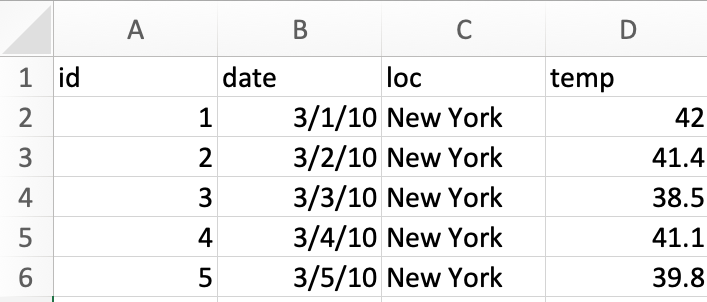
\includegraphics[width=300px]{images/example-data-type}

We read this data into R as below.

\begin{Shaded}
\begin{Highlighting}[]
\FunctionTok{library}\NormalTok{(readxl)}
\NormalTok{df }\OtherTok{\textless{}{-}} \FunctionTok{read\_excel}\NormalTok{(}\StringTok{"data/example{-}data{-}type.xlsx"}\NormalTok{)}
\end{Highlighting}
\end{Shaded}

Below is a print out of the data object. Are there any issues here?

\begin{Shaded}
\begin{Highlighting}[]
\NormalTok{df}
\end{Highlighting}
\end{Shaded}

\begin{verbatim}
## # A tibble: 5 x 4
##      id date                loc       temp
##   <dbl> <dttm>              <chr>    <dbl>
## 1     1 2010-01-03 00:00:00 New York  42  
## 2     2 2010-02-03 00:00:00 New York  41.4
## 3     3 2010-03-03 00:00:00 New York  38.5
## 4     4 2010-04-03 00:00:00 New York  41.1
## 5     5 2010-05-03 00:00:00 New York  39.8
\end{verbatim}

In the United States, it is common to use the date format MM/DD/YYYY while the rest of the world commonly use DD/MM/YYYY or YYYY/MM/DD. It is highly probable that the dates are 1st-5th March and not 3rd of Jan-May. You can \textbf{validate data with external sources}, e.g.~say the temperature at New York during the two choices suggest that the dates are 1st-5th March.

The benefit of working with data grounded in the real world process is that there are generally means to sanity check. You can robustify your workflow by ensuring that you have an explicit check for the expected data type (and values) in your code.

In the code below, we write our expected types and further coerce some data types to what we want.

\begin{Shaded}
\begin{Highlighting}[]
\FunctionTok{library}\NormalTok{(tidyverse)}
\end{Highlighting}
\end{Shaded}

\begin{verbatim}
## Warning: package 'tidyverse' was built under R version 4.0.2
\end{verbatim}

\begin{verbatim}
## -- Attaching packages --------------------------------------- tidyverse 1.3.1 --
\end{verbatim}

\begin{verbatim}
## v ggplot2 3.3.3     v purrr   0.3.4
## v tibble  3.1.1     v dplyr   1.0.6
## v tidyr   1.1.3     v stringr 1.4.0
## v readr   1.4.0     v forcats 0.5.1
\end{verbatim}

\begin{verbatim}
## Warning: package 'tibble' was built under R version 4.0.2
\end{verbatim}

\begin{verbatim}
## Warning: package 'tidyr' was built under R version 4.0.2
\end{verbatim}

\begin{verbatim}
## Warning: package 'readr' was built under R version 4.0.2
\end{verbatim}

\begin{verbatim}
## Warning: package 'dplyr' was built under R version 4.0.2
\end{verbatim}

\begin{verbatim}
## Warning: package 'forcats' was built under R version 4.0.2
\end{verbatim}

\begin{verbatim}
## -- Conflicts ------------------------------------------ tidyverse_conflicts() --
## x dplyr::filter() masks stats::filter()
## x dplyr::lag()    masks stats::lag()
\end{verbatim}

\begin{Shaded}
\begin{Highlighting}[]
\FunctionTok{read\_excel}\NormalTok{(}\StringTok{"data/example{-}data{-}type.xlsx"}\NormalTok{, }
                   \AttributeTok{col\_types =} \FunctionTok{c}\NormalTok{(}\StringTok{"text"}\NormalTok{, }\StringTok{"date"}\NormalTok{, }\StringTok{"text"}\NormalTok{, }\StringTok{"numeric"}\NormalTok{)) }\SpecialCharTok{\%\textgreater{}\%}
  \FunctionTok{mutate}\NormalTok{(}\AttributeTok{id =} \FunctionTok{as.factor}\NormalTok{(id),}
         \AttributeTok{date =} \FunctionTok{as.character}\NormalTok{(date),}
         \AttributeTok{date =} \FunctionTok{as.Date}\NormalTok{(date, }\AttributeTok{format =} \StringTok{"\%Y{-}\%d{-}\%m"}\NormalTok{))}
\end{Highlighting}
\end{Shaded}

\begin{verbatim}
## # A tibble: 5 x 4
##   id    date       loc       temp
##   <fct> <date>     <chr>    <dbl>
## 1 1     2010-03-01 New York  42  
## 2 2     2010-03-02 New York  41.4
## 3 3     2010-03-03 New York  38.5
## 4 4     2010-03-04 New York  41.1
## 5 5     2010-03-05 New York  39.8
\end{verbatim}

\begin{Shaded}
\begin{Highlighting}[]
\FunctionTok{read\_csv}\NormalTok{(}\StringTok{"data/example{-}data{-}type.csv"}\NormalTok{,}
         \AttributeTok{col\_types =} \FunctionTok{cols}\NormalTok{(}\AttributeTok{id =} \FunctionTok{col\_factor}\NormalTok{(),}
                          \AttributeTok{date =} \FunctionTok{col\_date}\NormalTok{(}\AttributeTok{format =} \StringTok{"\%m/\%d/\%y"}\NormalTok{),}
                          \AttributeTok{loc =} \FunctionTok{col\_character}\NormalTok{(),}
                          \AttributeTok{temp =} \FunctionTok{col\_double}\NormalTok{()))}
\end{Highlighting}
\end{Shaded}

\begin{verbatim}
## # A tibble: 5 x 4
##   id    date       loc       temp
##   <fct> <date>     <chr>    <dbl>
## 1 1     2010-03-01 New York  42  
## 2 2     2010-03-02 New York  41.4
## 3 3     2010-03-03 New York  38.5
## 4 4     2010-03-04 New York  41.1
## 5 5     2010-03-05 New York  39.8
\end{verbatim}

The checks (or coercions) ensure that even if the data are updated, you can have some confidence that any data type error will be picked up before further analysis.

\hypertarget{checking-the-data-quality}{%
\subsection{Checking the data quality}\label{checking-the-data-quality}}

Numerical or graphical summaries, or even just eye-balling the data, helps to uncover some data quality issues. Do you see any issues for the data below?

\begin{Shaded}
\begin{Highlighting}[]
\NormalTok{df2 }\OtherTok{\textless{}{-}} \FunctionTok{read\_csv}\NormalTok{(}\StringTok{"data/example{-}data{-}quality.csv"}\NormalTok{,}
                \AttributeTok{col\_types =} \FunctionTok{cols}\NormalTok{(}\AttributeTok{id =} \FunctionTok{col\_factor}\NormalTok{(),}
                                 \AttributeTok{date =} \FunctionTok{col\_date}\NormalTok{(}\AttributeTok{format =} \StringTok{"\%m/\%d/\%y"}\NormalTok{),}
                                 \AttributeTok{loc =} \FunctionTok{col\_character}\NormalTok{(),}
                                 \AttributeTok{temp =} \FunctionTok{col\_double}\NormalTok{()))}
\NormalTok{df2}
\end{Highlighting}
\end{Shaded}

\begin{verbatim}
## # A tibble: 9 x 4
##   id    date       loc        temp
##   <fct> <date>     <chr>     <dbl>
## 1 1     2010-03-01 New York   42  
## 2 2     2010-03-02 New York   41.4
## 3 3     2010-03-03 New York   38.5
## 4 4     2010-03-04 New York   41.1
## 5 5     2010-03-05 New York   39.8
## 6 6     2020-03-01 Melbourne  30.6
## 7 7     2020-03-02 Melbourne  17.9
## 8 8     2020-03-03 Melbourne  18.6
## 9 9     2020-03-04 <NA>       21.3
\end{verbatim}

There is a missing value in \texttt{loc}. Temperature is in Farenheit for New York but Celsius in Melbourne. You can find this out again using external sources.

Consider the soybean study conducted in Brazil (cite Lehner 2016). This study collected multiple traits of soybeans grown at multiple locations over years.

\begin{Shaded}
\begin{Highlighting}[]
\FunctionTok{library}\NormalTok{(naniar)}
\FunctionTok{data}\NormalTok{(}\StringTok{"lehner.soybeanmold"}\NormalTok{, }\AttributeTok{package =} \StringTok{"agridat"}\NormalTok{)}
\FunctionTok{vis\_miss}\NormalTok{(lehner.soybeanmold)}
\end{Highlighting}
\end{Shaded}

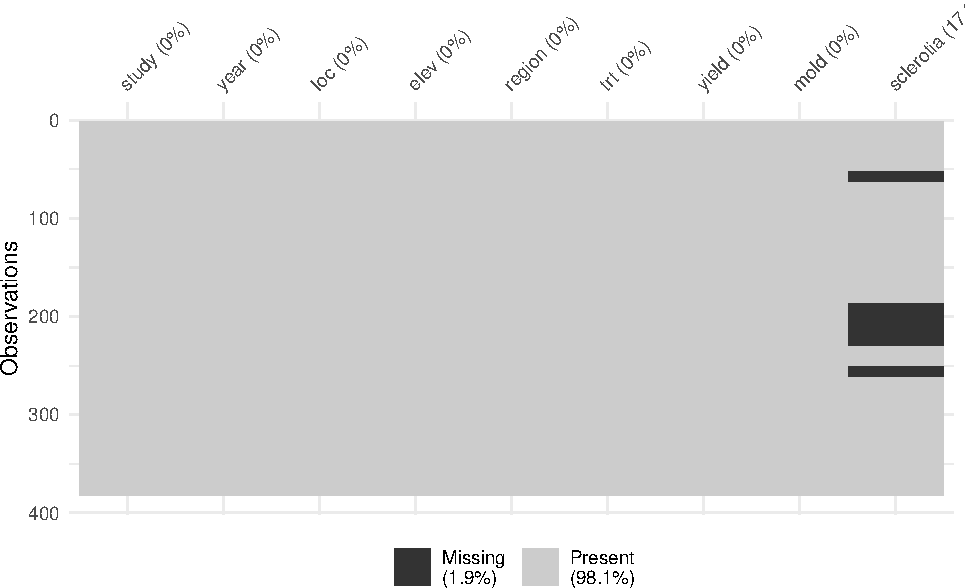
\includegraphics{eda-book_files/figure-latex/unnamed-chunk-8-1.pdf}

Inspecting the data reveals that there are a number of missing values for sclerotia and these values do not necessary appear missing at random. We could check if observational units that are missing values for sclerotia, have different yield say.

\begin{Shaded}
\begin{Highlighting}[]
\FunctionTok{ggplot}\NormalTok{(lehner.soybeanmold, }\FunctionTok{aes}\NormalTok{(sclerotia, yield)) }\SpecialCharTok{+}
  \FunctionTok{geom\_miss\_point}\NormalTok{()}
\end{Highlighting}
\end{Shaded}

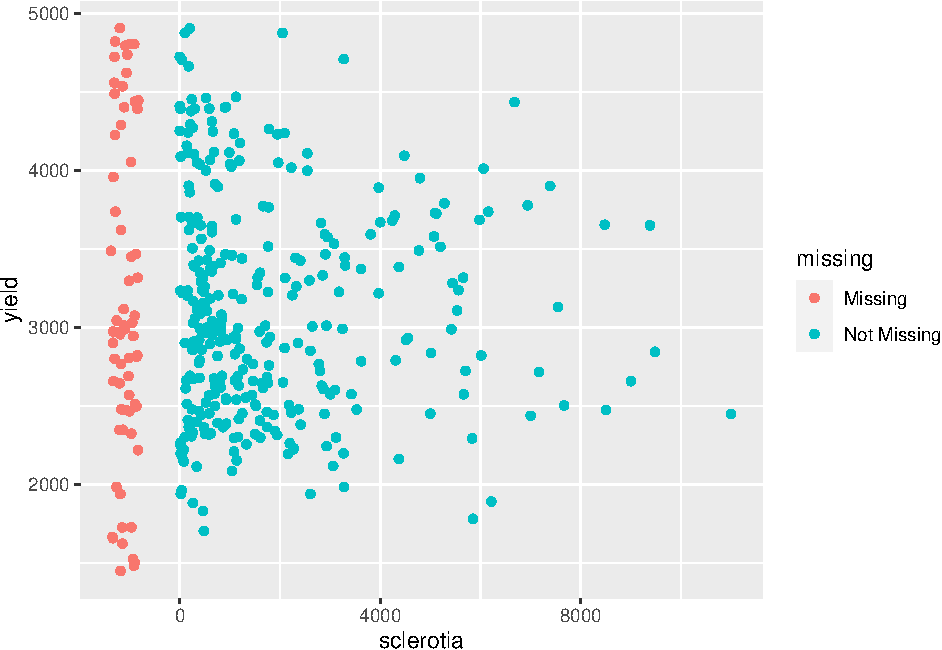
\includegraphics{eda-book_files/figure-latex/unnamed-chunk-9-1.pdf}

We could also compare the new data with old data.

\begin{Shaded}
\begin{Highlighting}[]
\FunctionTok{library}\NormalTok{(inspectdf)}
\end{Highlighting}
\end{Shaded}

\begin{verbatim}
## Warning: package 'inspectdf' was built under R version 4.0.2
\end{verbatim}

\begin{Shaded}
\begin{Highlighting}[]
\NormalTok{soy\_old }\OtherTok{\textless{}{-}}\NormalTok{ lehner.soybeanmold }\SpecialCharTok{\%\textgreater{}\%}
  \FunctionTok{filter}\NormalTok{(year }\SpecialCharTok{\%in\%} \DecValTok{2010}\SpecialCharTok{:}\DecValTok{2011}\NormalTok{)}
\NormalTok{soy\_new }\OtherTok{\textless{}{-}}\NormalTok{ lehner.soybeanmold }\SpecialCharTok{\%\textgreater{}\%}
  \FunctionTok{filter}\NormalTok{(year }\SpecialCharTok{==} \DecValTok{2012}\NormalTok{)}

\FunctionTok{inspect\_cor}\NormalTok{(soy\_old, soy\_new) }\SpecialCharTok{\%\textgreater{}\%}
  \FunctionTok{show\_plot}\NormalTok{()}
\end{Highlighting}
\end{Shaded}

\begin{verbatim}
## Warning: Columns with 0 variance found: year
\end{verbatim}

\begin{verbatim}
## Warning in grid.Call(C_textBounds, as.graphicsAnnot(x$label), x$x, x$y, :
## conversion failure on 'Comparison of ρ between df::soy_old and soy_new' in
## 'mbcsToSbcs': dot substituted for <cf>
\end{verbatim}

\begin{verbatim}
## Warning in grid.Call(C_textBounds, as.graphicsAnnot(x$label), x$x, x$y, :
## conversion failure on 'Comparison of ρ between df::soy_old and soy_new' in
## 'mbcsToSbcs': dot substituted for <81>
\end{verbatim}

\begin{verbatim}
## Warning in grid.Call(C_textBounds, as.graphicsAnnot(x$label), x$x, x$y, :
## conversion failure on 'Comparison of ρ between df::soy_old and soy_new' in
## 'mbcsToSbcs': dot substituted for <cf>
\end{verbatim}

\begin{verbatim}
## Warning in grid.Call(C_textBounds, as.graphicsAnnot(x$label), x$x, x$y, :
## conversion failure on 'Comparison of ρ between df::soy_old and soy_new' in
## 'mbcsToSbcs': dot substituted for <81>
\end{verbatim}

\begin{verbatim}
## Warning in grid.Call(C_textBounds, as.graphicsAnnot(x$label), x$x, x$y, :
## conversion failure on 'Comparison of ρ between df::soy_old and soy_new' in
## 'mbcsToSbcs': dot substituted for <cf>
\end{verbatim}

\begin{verbatim}
## Warning in grid.Call(C_textBounds, as.graphicsAnnot(x$label), x$x, x$y, :
## conversion failure on 'Comparison of ρ between df::soy_old and soy_new' in
## 'mbcsToSbcs': dot substituted for <81>
\end{verbatim}

\begin{verbatim}
## Warning in grid.Call(C_textBounds, as.graphicsAnnot(x$label), x$x, x$y, :
## conversion failure on 'Comparison of ρ between df::soy_old and soy_new' in
## 'mbcsToSbcs': dot substituted for <cf>
\end{verbatim}

\begin{verbatim}
## Warning in grid.Call(C_textBounds, as.graphicsAnnot(x$label), x$x, x$y, :
## conversion failure on 'Comparison of ρ between df::soy_old and soy_new' in
## 'mbcsToSbcs': dot substituted for <81>
\end{verbatim}

\begin{verbatim}
## Warning in grid.Call(C_textBounds, as.graphicsAnnot(x$label), x$x, x$y, :
## conversion failure on 'Comparison of ρ between df::soy_old and soy_new' in
## 'mbcsToSbcs': dot substituted for <cf>
\end{verbatim}

\begin{verbatim}
## Warning in grid.Call(C_textBounds, as.graphicsAnnot(x$label), x$x, x$y, :
## conversion failure on 'Comparison of ρ between df::soy_old and soy_new' in
## 'mbcsToSbcs': dot substituted for <81>
\end{verbatim}

\begin{verbatim}
## Warning in grid.Call(C_textBounds, as.graphicsAnnot(x$label), x$x, x$y, :
## conversion failure on 'Comparison of ρ between df::soy_old and soy_new' in
## 'mbcsToSbcs': dot substituted for <cf>
\end{verbatim}

\begin{verbatim}
## Warning in grid.Call(C_textBounds, as.graphicsAnnot(x$label), x$x, x$y, :
## conversion failure on 'Comparison of ρ between df::soy_old and soy_new' in
## 'mbcsToSbcs': dot substituted for <81>
\end{verbatim}

\begin{verbatim}
## Warning in grid.Call(C_textBounds, as.graphicsAnnot(x$label), x$x, x$y, :
## conversion failure on 'Comparison of ρ between df::soy_old and soy_new' in
## 'mbcsToSbcs': dot substituted for <cf>
\end{verbatim}

\begin{verbatim}
## Warning in grid.Call(C_textBounds, as.graphicsAnnot(x$label), x$x, x$y, :
## conversion failure on 'Comparison of ρ between df::soy_old and soy_new' in
## 'mbcsToSbcs': dot substituted for <81>
\end{verbatim}

\begin{verbatim}
## Warning in grid.Call.graphics(C_text, as.graphicsAnnot(x$label), x$x, x$y, :
## conversion failure on 'Comparison of ρ between df::soy_old and soy_new' in
## 'mbcsToSbcs': dot substituted for <cf>
\end{verbatim}

\begin{verbatim}
## Warning in grid.Call.graphics(C_text, as.graphicsAnnot(x$label), x$x, x$y, :
## conversion failure on 'Comparison of ρ between df::soy_old and soy_new' in
## 'mbcsToSbcs': dot substituted for <81>
\end{verbatim}

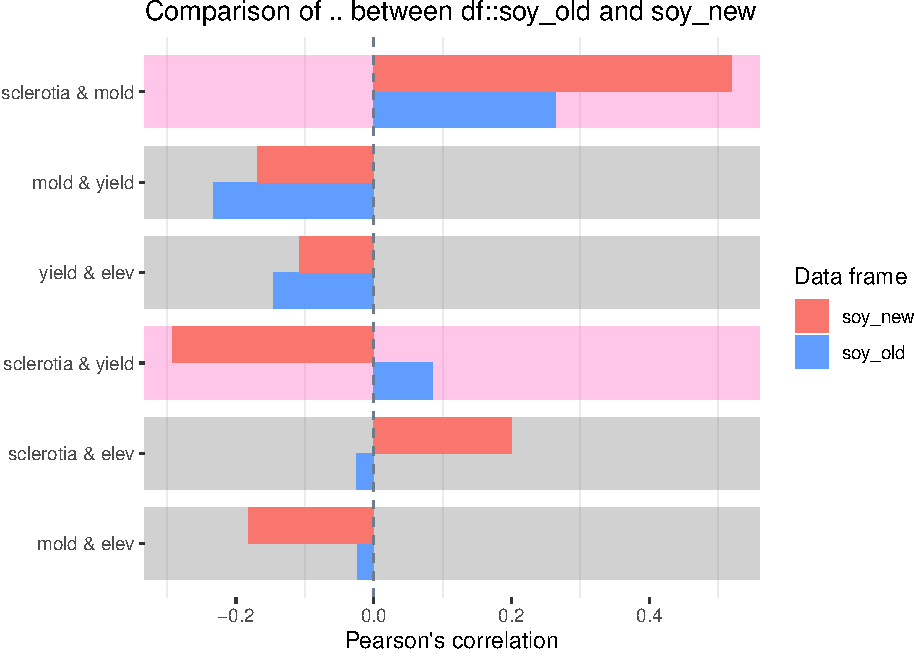
\includegraphics{eda-book_files/figure-latex/unnamed-chunk-10-1.pdf}

\hypertarget{check-on-data-collection-method}{%
\subsection{Check on data collection method}\label{check-on-data-collection-method}}

Next we study the data from ABS that shows the total number of people employed in a given month from February 1976 to December 2019 using the original time series.

\begin{Shaded}
\begin{Highlighting}[]
\FunctionTok{library}\NormalTok{(readabs)}
\end{Highlighting}
\end{Shaded}

\begin{verbatim}
## Warning: package 'readabs' was built under R version 4.0.2
\end{verbatim}

\begin{Shaded}
\begin{Highlighting}[]
\NormalTok{employed }\OtherTok{\textless{}{-}} \FunctionTok{read\_abs}\NormalTok{(}\AttributeTok{series\_id =} \StringTok{"A84423085A"}\NormalTok{) }\SpecialCharTok{\%\textgreater{}\%} 
  \FunctionTok{mutate}\NormalTok{(}\AttributeTok{month =}\NormalTok{ lubridate}\SpecialCharTok{::}\FunctionTok{month}\NormalTok{(date),}
         \AttributeTok{year =} \FunctionTok{factor}\NormalTok{(lubridate}\SpecialCharTok{::}\FunctionTok{year}\NormalTok{(date))) }\SpecialCharTok{\%\textgreater{}\%} 
  \FunctionTok{filter}\NormalTok{(year }\SpecialCharTok{!=} \StringTok{"2020"}\NormalTok{) }\SpecialCharTok{\%\textgreater{}\%} 
  \FunctionTok{select}\NormalTok{(date, month, year, value) }
\end{Highlighting}
\end{Shaded}

Do you notice anything?

\begin{Shaded}
\begin{Highlighting}[]
\NormalTok{employed  }\SpecialCharTok{\%\textgreater{}\%} 
  \FunctionTok{ggplot}\NormalTok{(}\FunctionTok{aes}\NormalTok{(month, value, }\AttributeTok{color =}\NormalTok{ year)) }\SpecialCharTok{+} 
  \FunctionTok{geom\_line}\NormalTok{() }\SpecialCharTok{+} 
  \FunctionTok{ggtitle}\NormalTok{(}\StringTok{"1978 Feb {-} 2019 Dec"}\NormalTok{) }
\end{Highlighting}
\end{Shaded}

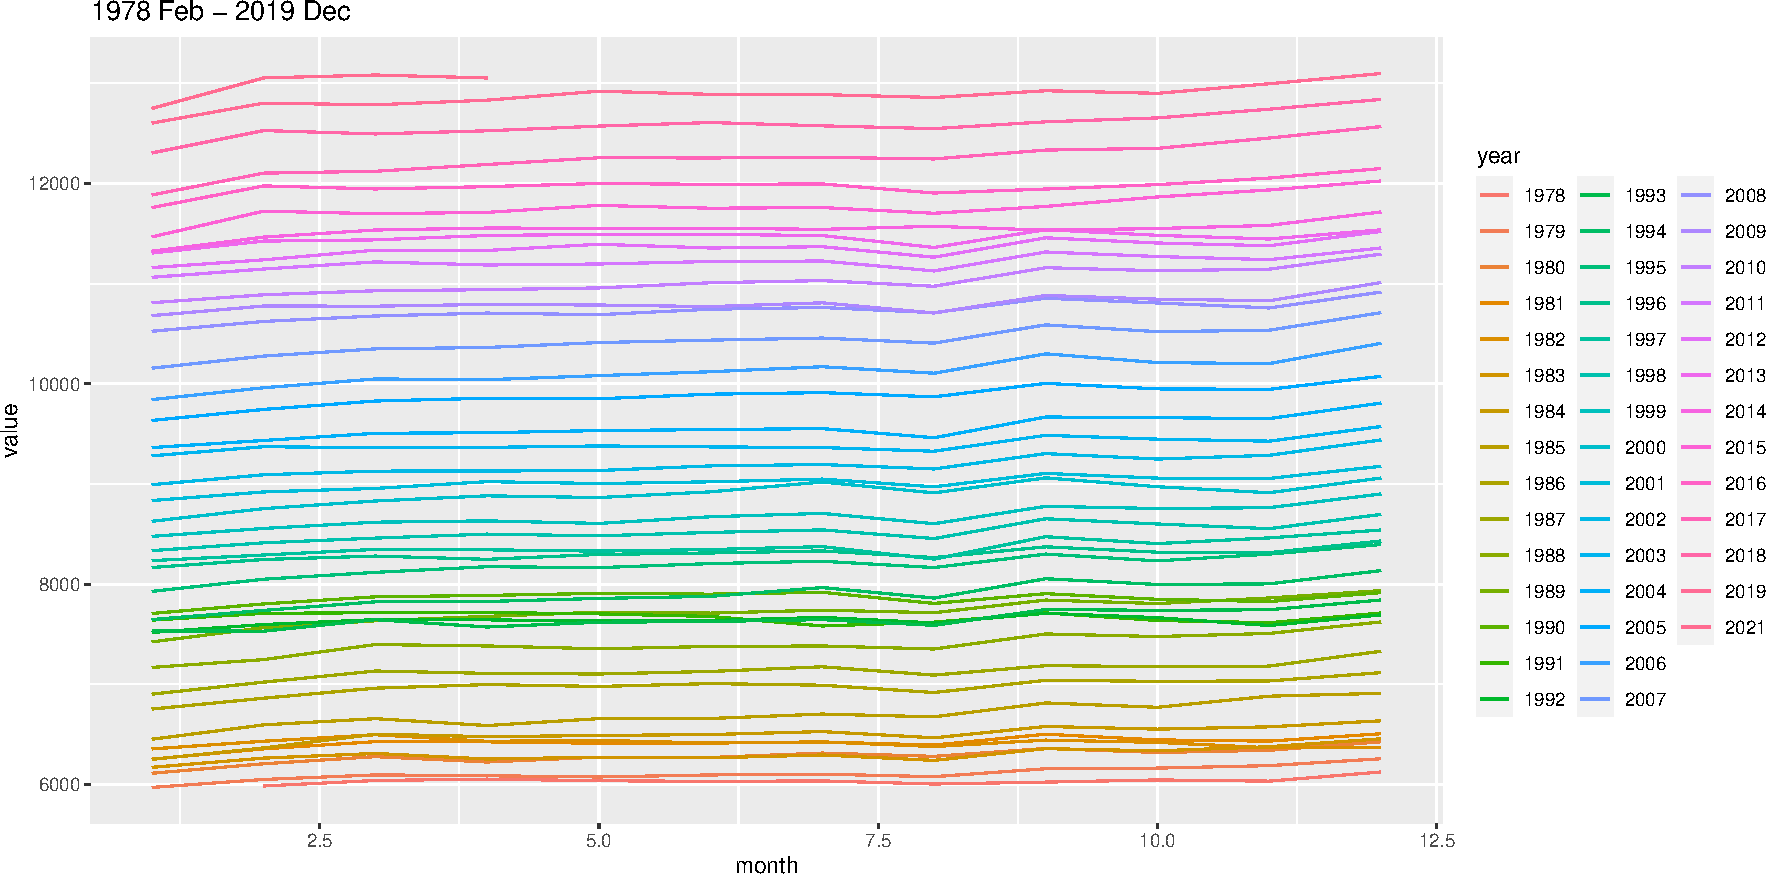
\includegraphics{eda-book_files/figure-latex/unnamed-chunk-12-1.pdf}

Why do you think the number of people employed is going up each year?

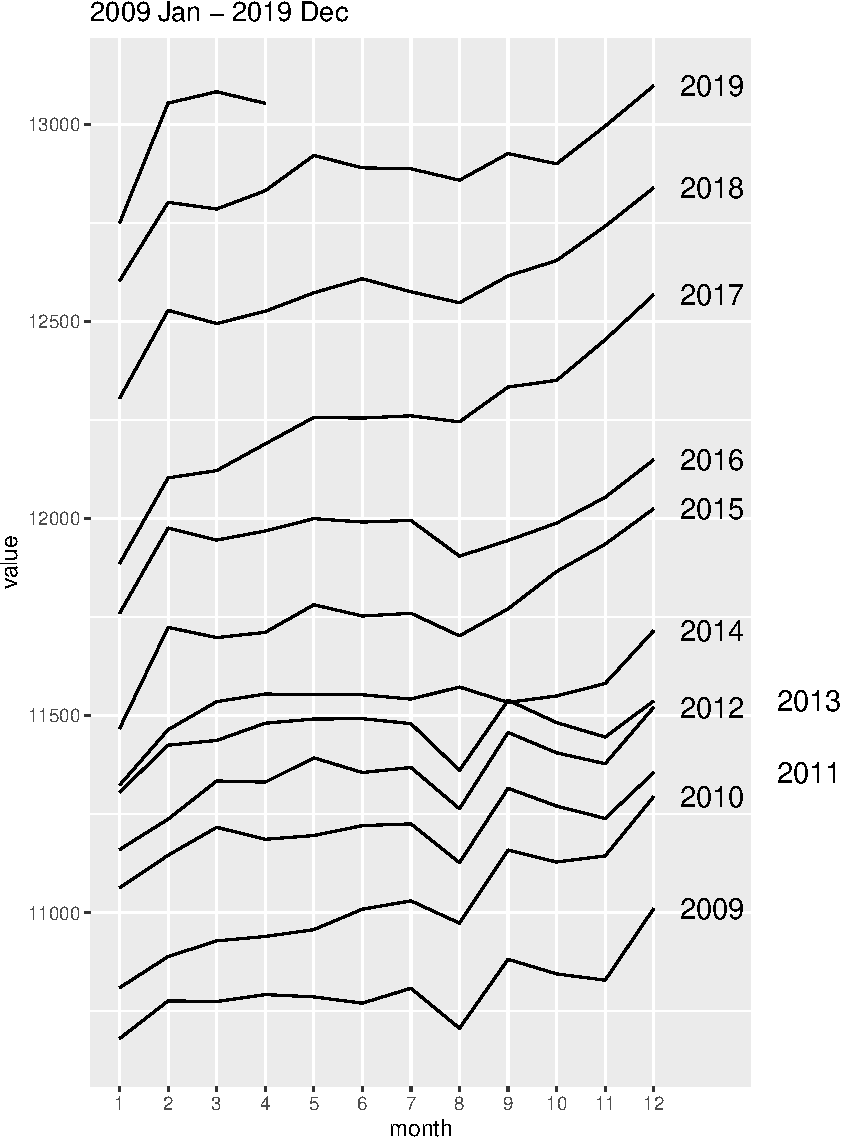
\includegraphics{eda-book_files/figure-latex/unnamed-chunk-13-1.pdf}

There's a suspicious change in August numbers from 2014.

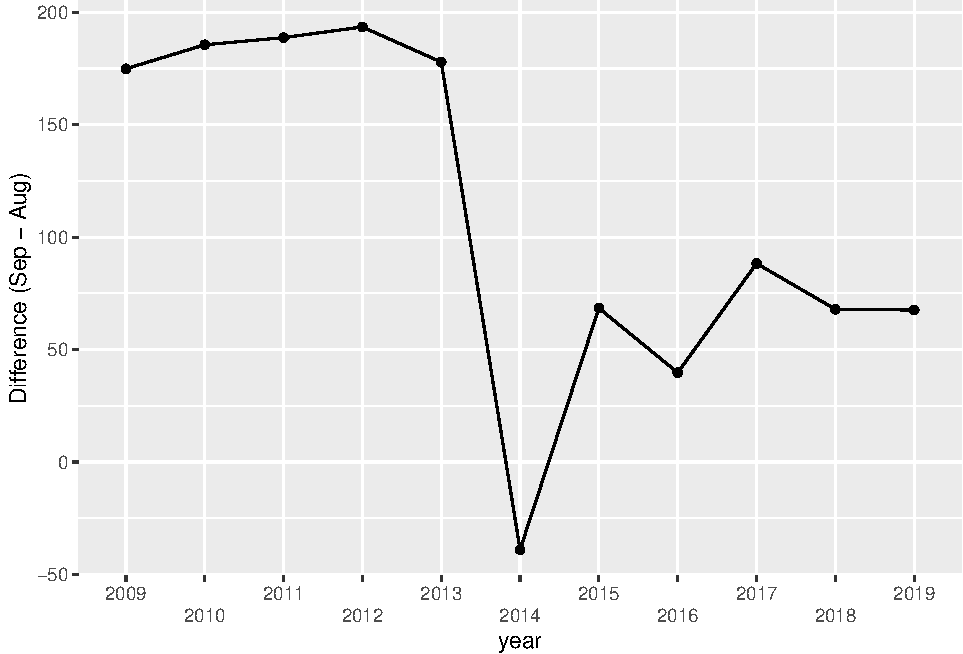
\includegraphics{eda-book_files/figure-latex/unnamed-chunk-14-1.pdf}

A potential explanation for this is that there was a \emph{change in the survey from 2014}. Also see \url{https://robjhyndman.com/hyndsight/abs-seasonal-adjustment-2/}

\textbf{Check if the \emph{data collection} method has been consistent.}

\hypertarget{check-for-experimental-data}{%
\subsection{Check for experimental data}\label{check-for-experimental-data}}

For experimental data, there would generally be some descriptions that include the experimental layout and any randomisation process of controlled variables (e.g.~treatments) to units.

Consider the experiment below. The experiment tests the effects of 9 fertilizer treatments on the yield of brussel sprouts on a field laid out in a rectangular array of 6 rows and 8 columns.

\begin{Shaded}
\begin{Highlighting}[]
\NormalTok{df3 }\OtherTok{\textless{}{-}} \FunctionTok{read\_csv}\NormalTok{(}\StringTok{"data/example{-}experimental{-}data.csv"}\NormalTok{, }
                \AttributeTok{col\_types =} \FunctionTok{cols}\NormalTok{(}\AttributeTok{row =} \FunctionTok{col\_factor}\NormalTok{(),}
                                 \AttributeTok{col =} \FunctionTok{col\_factor}\NormalTok{(),}
                                 \AttributeTok{yield =} \FunctionTok{col\_double}\NormalTok{(),}
                                 \AttributeTok{trt =} \FunctionTok{col\_factor}\NormalTok{(),}
                                 \AttributeTok{block =} \FunctionTok{col\_factor}\NormalTok{()))}
\end{Highlighting}
\end{Shaded}

\begin{verbatim}
## Warning: package 'colorspace' was built under R version 4.0.2
\end{verbatim}

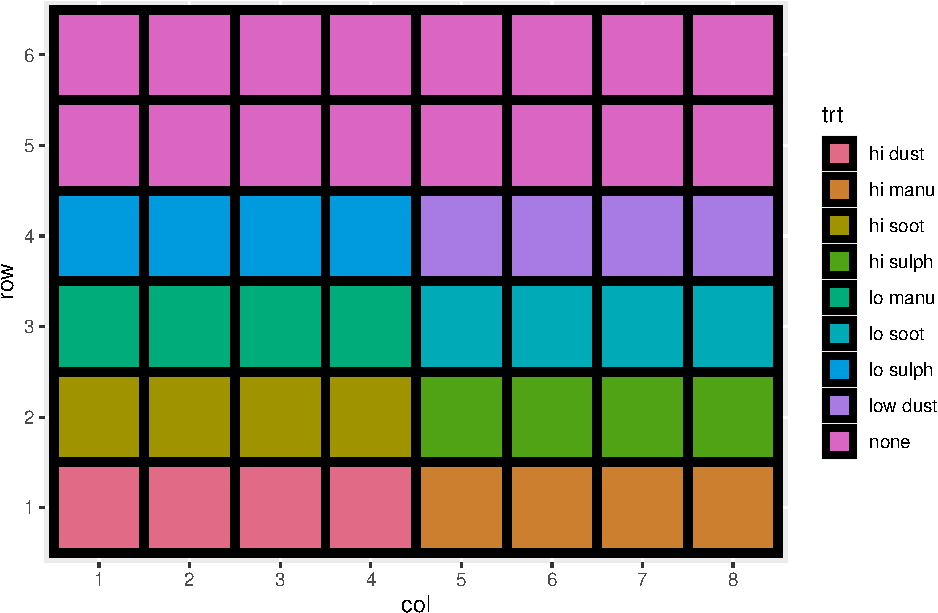
\includegraphics{eda-book_files/figure-latex/unnamed-chunk-16-1.pdf} 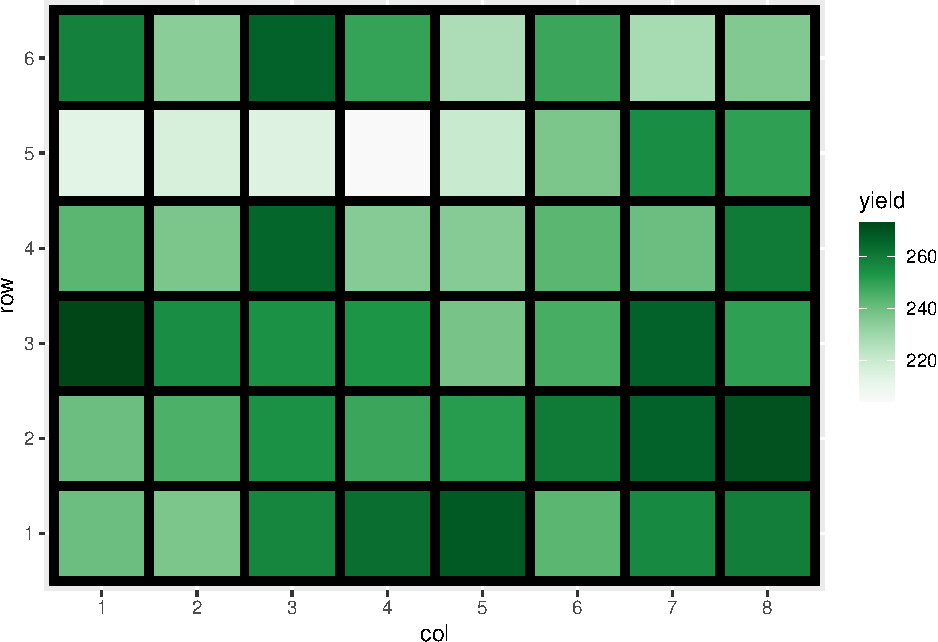
\includegraphics{eda-book_files/figure-latex/unnamed-chunk-16-2.pdf}

\begin{Shaded}
\begin{Highlighting}[]
\NormalTok{df3 }\SpecialCharTok{\%\textgreater{}\%} 
  \FunctionTok{mutate}\NormalTok{(}\AttributeTok{trt =} \FunctionTok{fct\_reorder}\NormalTok{(trt, yield)) }\SpecialCharTok{\%\textgreater{}\%} 
  \FunctionTok{ggplot}\NormalTok{(}\FunctionTok{aes}\NormalTok{(trt, yield)) }\SpecialCharTok{+} 
  \FunctionTok{geom\_point}\NormalTok{(}\AttributeTok{size =} \DecValTok{4}\NormalTok{, }\AttributeTok{alpha =} \DecValTok{1} \SpecialCharTok{/} \DecValTok{2}\NormalTok{) }\SpecialCharTok{+} 
  \FunctionTok{guides}\NormalTok{(}\AttributeTok{x =} \FunctionTok{guide\_axis}\NormalTok{(}\AttributeTok{n.dodge =} \DecValTok{2}\NormalTok{))}
\end{Highlighting}
\end{Shaded}

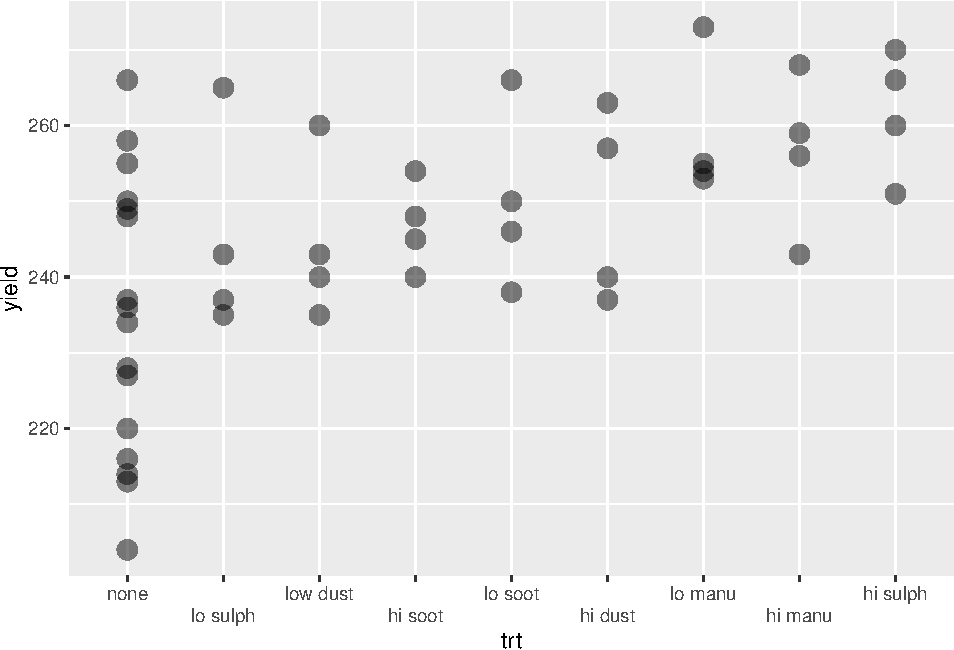
\includegraphics{eda-book_files/figure-latex/unnamed-chunk-17-1.pdf}

High sulphur and high manure seems to best for the yield of brussel sprouts. Any issues here?

\hypertarget{model-formulation}{%
\section{Model formulation}\label{model-formulation}}

\begin{info}
Note: there are variety of ways to do IDA and you don't need to
prescribe to what we show you.
\end{info}

\hypertarget{working-with-a-single-variable}{%
\chapter{Working with a single variable}\label{working-with-a-single-variable}}

making transformations, detecting outliers, using robust statistics

\hypertarget{bivariate-dependencies-and-relationships}{%
\chapter{Bivariate dependencies and relationships}\label{bivariate-dependencies-and-relationships}}

transformations to linearise

\hypertarget{going-beyond-two-variables}{%
\chapter{Going beyond two variables}\label{going-beyond-two-variables}}

exploring high dimensions

\hypertarget{making-comparisons-between-groups-and-strata}{%
\chapter{Making comparisons between groups and strata}\label{making-comparisons-between-groups-and-strata}}

\hypertarget{sculpting-data-using-models}{%
\chapter{Sculpting data using models}\label{sculpting-data-using-models}}

checking assumptions, co-dependency and performing diagnostics

\hypertarget{exploring-data-having-a-space-and-time-context}{%
\chapter{Exploring data having a space and time context}\label{exploring-data-having-a-space-and-time-context}}

\hypertarget{is-what-you-see-really-there}{%
\chapter{Is what you see really there?}\label{is-what-you-see-really-there}}

Using computational tools to determine whether what is seen in the data can be assumed to apply more broadly

\hypertarget{final-words}{%
\chapter{Final words}\label{final-words}}

  \bibliography{book.bib,packages.bib}

\end{document}
